\section{Architectural requirements}






\subsection{Quality Attributes workshop}
In this section we will present 8 phases of the QAW. Despite that a workshop is not held we still see clear benefits by using this model namely to determine the qualities for the electronic voting application before it is implemented. We are well aware that the outcome isn't perfect. 
\begin{description}
    \item [QAW Presentation and Introductions]
        QAW facilitators describe the motivation for the QAW and explain each step of the method. 
    
    \item [Business/Mission Presentation]    
        A representative of the stakeholder community presents the business and/or programmatic drivers for the system.
    
    \item [Architectural Plan Presentation]
        A technical stakeholder presents the system architectural plans as they stand with respect to early documents, such as high-level system descriptions, context drawings, or other artifacts that describe some of the system's technical details.
    
    \item [Identification of Architectural Drivers]
     Architectural drivers often include high-level requirements, business/mission concerns, goals and objectives, and various quality attributes. During this step, the facilitators and stakeholders reach a consensus about which drivers are key to the system.
          
    
    \item [Scenario Brainstorm]
        Stakeholders generate real-world scenarios for the system. Scenarios comprise a related stimulus, an environmental condition, and a response. Facilitators ensure that at least one scenario addresses each of the architectural drivers identified in Step 4.
         
    \item [Consolidation] 
        Scenarios that are similar in content are consolidated.
    
    \item [Prioritization] 
  Stakeholders prioritize the scenarios through a voting process. 
    
    \item [Refinement]
        The top four or five scenarios are further clarified and the following are described:
        \begin{enumerate}
            \item the business/programmatic goals that are affected by those scenarios
            \item the relevant quality attributes associated with those scenarios   
        \end{enumerate}

   

\end{description}




\subsubsection{2. Business / mission presentation}
In this phase we will present our case.
 
\subsubsection{3. Architectural Plan Presentation}
We will use this step to wrap up our first iteration for a high level overview of the system. This first overview is all based on the knowledge we got from the first part. We illustrate this overview through a component connector view. This viewpoint is concerned with the run-time functionality of the system.  At this point we have a component for a voter, tallier, observer, bulletinboard and a registration process. We see the voter, tallier and the observers as clients and as active processes which all are communicating with the  bulletinboard. Therefor their must be a connector between the clients and bulletinboard. The purpose of the registration authority is that every active participant must be registered through some registration authority before they can attend the electronic voting election. 

\begin{center}
     \makebox[\textwidth]{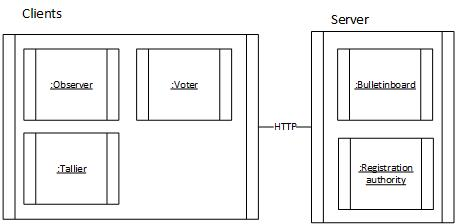
\includegraphics[scale=0.90]{CC_View_2.jpg}}
\end{center}

\subsubsection{4. Identify architectural drivers}
The purpose of this step is to identify architectural drivers. Architectural drivers are the keys to realizing quality attribute goals for the system. The architectural drivers are often found through requirements and business goals. We found architectural drivers by reflection and discussion against the security requirements of earlier described electronic voting application. Based on our architectural drivers, we begin to see the following quality attributes.\\


\begin{table}[H]
\centering
\begin{tabular}{|l|l|}
\hline
\multicolumn{2}{|l|}{Voters point of view}                \\ \hline
Usability    & The system should be easy to use for a voter                   \\ \hline
Availability    & \begin{tabular}[c]{@{}l@{}}The system should be reliability and should \\ give detailed feedback \end{tabular}   \\ \hline 
Availability & The system should be available when needed                     \\ \hline
Interoperability         & \begin{tabular}[c]{@{}l@{}} A voter should be able to cast a vote \\ from a given device with a internet \\ connection\end{tabular}                                                                   \\ \hline

\end{tabular}
\caption{Voters point of view}
\label{my-label}
\end{table}


\begin{table}[H]
\centering
\begin{tabular}{|l|l|}
\hline
\multicolumn{2}{|l|}{Robustness}                                                                                                                                                                        \\ \hline
Performence         & \begin{tabular}[c]{@{}l@{}}Should be able to handle a large amount \\ of user within a reasonable time\end{tabular}                                                                   \\ \hline
Testability      & \begin{tabular}[c]{@{}l@{}}Given the nature of systems complexity it\\ should be easily testable to ensure \\ robustness and reliability\end{tabular}                                 \\ \hline
Security         & \begin{tabular}[c]{@{}l@{}}The integrity should withhold even though \\ if cheating occurs.\end{tabular}                                                                             \\ \hline
\multicolumn{2}{|l|}{Universal verifiability}                                                                                                                                                           \\ \hline
Interoperability & \begin{tabular}[c]{@{}l@{}}Not only participant but also passive observers \\ should be able to validate through out the \\ election and afterwards.\end{tabular}           \\ \hline

\multicolumn{2}{|l|}{Future proof}                                                                                                                                                                      \\ \hline
Modifiable       & \begin{tabular}[c]{@{}l@{}}Only a registered user should be able to vote. \\ This registration should be easily replaceable \\ depending on the nature of the election.\end{tabular} \\ \hline
Modifiable       & \begin{tabular}[c]{@{}l@{}}The system should modifiable such that\\  core elements are replaceable\end{tabular}                                                                      \\ \hline
\end{tabular}
\caption{Owners point of view}
\label{my-label}
\end{table}


\subsubsection{5. Scenario brainstorming}
The purpose of this step is to design quality attribute scenarios (QAS), based on our AD's. That is, here we form QAS in a form such as Bass et al. Form so there is clear stimulus and clear response measure.

\begin{table}[H]
\centering

\label{my-label}
\begin{tabular}{|l|l|l|}
\hline
Scenario \#      & Description                                                                                                                                                                                                                                                                          & Votes \\ \hline
1        & \begin{tabular}[c]{@{}l@{}}A user casts a vote under \\ runtime and the PVSS client registers\\ the vote with a confirm message, within\\ 5 seconds.\end{tabular}                                                                                                                    &       \\ \hline
2     & \begin{tabular}[c]{@{}l@{}}An internal crash occurs and the\\ Bulletin board is out of reach\\ during normal operation. The response\\ is that the error is logged and the \\ system is running in degraded mode.\\ The system should be up running\\ within 5 minutes.\end{tabular} &       \\ \hline
3 & \begin{tabular}[c]{@{}l@{}}A PVSS client cast a vote to the\\ Bulletin board from a given device\\ with internet connection  under runtime and\\ the system is updated and 100\% \\ of the information is exchanged \\ and processed correctly.\end{tabular}                                                                          &       \\ \hline
4 & \begin{tabular}[c]{@{}l@{}}An observer client validates\\ a vote from the the Bulletin board \\ under runtime. The validation is \\ processed, and the Bulletin board is\\ updated and 100\% of the information \\ is exchanged and processed correctly.\end{tabular} &       \\ \hline
5      & \begin{tabular}[c]{@{}l@{}}5 mill. users intiate their votes \\to the Bulletinboard \\ under normal operation.\\ The votes are processed and saved \\ with average latency of\\ 2 seconds.\end{tabular} &       \\ \hline
6      & \begin{tabular}[c]{@{}l@{}}An unitester should be able to\\ code a unit on the system\\ under development and the test suite\\ are executed  and result are captured\\ and 85\% of the system are coverage \\ within 3 hours.\end{tabular} &       \\ \hline
7       & \begin{tabular}[c]{@{}l@{}}A developer should be able to make a\\ change to the registration code under \\ runtime and the change are made and tested\\ within 3 hours.\end{tabular}                                                                                          &       \\ \hline
8       & \begin{tabular}[c]{@{}l@{}}A developer should be able to make a \\ change to the random number generator\\ code under runtime and the change are made\\ and tested within 3 hours.\end{tabular}                                                                                                   &       \\ \hline
9         & \begin{tabular}[c]{@{}l@{}}A cheater cast a invalid vote to the Bulletin\\ board under normal operation. All valid data\\ should be preserved and the system\\ should be able to detect invalid from \\ valid data before the total counting of \\ the votes.\end{tabular}           &       \\ \hline
10      & \begin{tabular}[c]{@{}l@{}}1000 transactions are initiates towards \\ the bulletin board under normal operation.\\ The transaction are processed and there are\\ a max latency of 5 seconds.\end{tabular}                                                                            &       \\ \hline
\end{tabular}
\caption{First step towards quality attributes scenarios}
\end{table}

\subsubsection{6. Scenario consideration}
The purpose of this step is to merge scenarios that have similar features. At the workshop there were no scenarios that could be merged.\\

\noindent
We merge the two architectural driver regarding availability. These two architectural drivers are closely related since the both are about the system performing the required functions without falling when needed.

\subsubsection{7. Scenario prioritization}
The purpose of this step is to draw up a priority list based on the total votes. The list is long but we will limit this thesis to focusing on a few and the rest we will comment. The list is prioritized based on the security requirements.

\begin{description}
    \item [Scenario 3 + 8]
        Since the PVSS is a public verifiable protocol, there will be a high focus on fulfilling the universal verifiability requirement. This means if there are invalid votes they should be detected through public verification. To achieve that we will create web application which can be access by everyone how has a device connected to the internet. 
    
    \item [Scenario 6 + 7]    
        To ensure eligibility and uniqueness there will be high focus on creating a flexible registration module which first of all ensures authentication and authorization such that only registered voters can vote and only have permissions to vote one time. But the module should be flexible enough to be change to integrate to other registration data. There wil be high focus on ensuring the fairness property regarding that none should be able to gain any knowledge of the outcome of the election. Also the uncoercibility property part regarding no one should be able to extract the value of a vote. Therefor the need to have a module which can generate/compute large numbers. The security can change over time and the need of computing larger numbers will therefor be a demand. The code should therefor be flexible if there is need for replacing the module with another number generator.  
        
    \item [Scenario 5]
        To ensure accuracy that final tally is computed correctly there will be high focus on ensuring the complex part of the code is testable.    
    
  \end{description}




\subsubsection{8. Scenario Refinement}
The purpose of this step is to form QAS based on Bass et al, where divide into source, stimulus, artifact, environment, response and response measure. 


\begin{table}[H]
\begin{center}
\begin{tabular}{|p{0.3cm}|p{2.5cm}|p{8cm}|}
  \hline
  \multicolumn{2}{|p{3cm}|}{\bfseries Scenario(s):} & \#  1: A PVSS client cast a vote to the Bulletin board from a given device with internet connection  under runtime and the system is updated and 100\% of the information is exchanged  and processed correctly\\
  \hline
  \multicolumn{2}{|p{3cm}|}{\bfseries Relevant Quality Attributes:} & Interoperability\\
  \hline
  \multirow{6}{*}{\begin{sideways}{\bfseries Scenario Parts}\end{sideways}}
  & {\bfseries Source:} & A webbrowser \\
  \cline{2-3}
  & {\bfseries Stimulus:} & Cast a vote \\
  \cline{2-3}
  & {\bfseries Artifact} &  Bulletinboard system \\
  \cline{2-3}
  & {\bfseries Environment:} &  Runtime \\
  \cline{2-3}
  & {\bfseries Response:} &  If the vote is valid it is accepted. If the vote is invalid it is rejected and the vote is removed from the Bulletinboard \\
  \cline{2-3}
  & {\bfseries Response Measure:} & 100 \% of the information is exchange and processed correctly \\
  \hline
\end{tabular}
\caption{Quality Attribute Scenario}
\end{center}
\end{table}


\begin{table}[H]
\begin{center}
\begin{tabular}{|p{0.3cm}|p{2.5cm}|p{8cm}|}
  \hline
  \multicolumn{2}{|p{3cm}|}{\bfseries Scenario(s):} & \#  2: A cheater cast a invalid vote to the Bulletin board under normal operation. All valid data should be preserved and the system should be able to detect invalid from  valid data before the total counting of the votes\\
  \hline
  \multicolumn{2}{|p{3cm}|}{\bfseries Relevant Quality Attributes:} & Security\\
  \hline
  \multirow{6}{*}{\begin{sideways}{\bfseries Scenario Parts}\end{sideways}}
  & {\bfseries Source:} & A cheater \\
  \cline{2-3}
  & {\bfseries Stimulus:} & Cast a invalid vote, with purpose of influencing the finale votes \\
  \cline{2-3}
  & {\bfseries Artifact} &  Bulletinboard system \\
  \cline{2-3}
  & {\bfseries Environment:} &  Runtime \\
  \cline{2-3}
  & {\bfseries Response:} &  If the vote is valid it is accepted. If the vote is invalid it is rejected and the vote is removed from the Bulletinboard \\
  \cline{2-3}
  & {\bfseries Response Measure:} & 100 \% of the information is exchange and processed correctly \\
  \hline
\end{tabular}
\caption{Quality Attribute Scenario}
\end{center}
\end{table}

\begin{table}[H]
\begin{center}
\begin{tabular}{|p{0.3cm}|p{2.5cm}|p{8cm}|}
  \hline
  \multicolumn{2}{|p{3cm}|}{\bfseries Scenario(s):} & \#  3: A developer should be able to make a change to the random number generator code under runtime and the change are made and tested within 3 hours. \\
  \hline
  \multicolumn{2}{|p{3cm}|}{\bfseries Relevant Quality Attributes:} & Modifiability\\
  \hline
  \multirow{6}{*}{\begin{sideways}{\bfseries Scenario Parts}\end{sideways}}
  & {\bfseries Source:} & Developer \\
  \cline{2-3}
  & {\bfseries Stimulus:} & Needs to replace the random generator \\
  \cline{2-3}
  & {\bfseries Artifact} &  Code \\
  \cline{2-3}
  & {\bfseries Environment:} &  Design time \\
  \cline{2-3}
  & {\bfseries Response:} &  Replacement made and Unit tested\\
  \cline{2-3}
  & {\bfseries Response Measure:} & In three hours\\
  \hline
\end{tabular}
\caption{Quality Attribute Scenario}
\end{center}
\end{table}

\begin{table}[H]
\begin{center}
\begin{tabular}{|p{0.3cm}|p{2.5cm}|p{8cm}|}
  \hline
  \multicolumn{2}{|p{3cm}|}{\bfseries Scenario(s):} & \#  4:A developer should be able to make a change to the registration code under runtime and the change are made and tested within 3 hours \\
  \hline
  \multicolumn{2}{|p{3cm}|}{\bfseries Relevant Quality Attributes:} & Modifiability\\
  \hline
  \multirow{6}{*}{\begin{sideways}{\bfseries Scenario Parts}\end{sideways}}
  & {\bfseries Source:} & Developer \\
  \cline{2-3}
  & {\bfseries Stimulus:} & Needs to replace the registration module \\
  \cline{2-3}
  & {\bfseries Artifact} &  Code \\
  \cline{2-3}
  & {\bfseries Environment:} &  Design time \\
  \cline{2-3}
  & {\bfseries Response:} &  Replacement made and Unit tested\\
  \cline{2-3}
  & {\bfseries Response Measure:} & In three hours\\
  \hline
\end{tabular}
\caption{Quality Attribute Scenario}
\end{center}
\end{table}

\begin{table}[H]
\begin{center}
\begin{tabular}{|p{0.3cm}|p{2.5cm}|p{8cm}|}
  \hline
  \multicolumn{2}{|p{3cm}|}{\bfseries Scenario(s):} & \#  5: 5 mill. users intiate votes to the Bulletinboard under normal operation. The votes are processed and saved with average latency of 2 seconds.\\
  \hline
  \multicolumn{2}{|p{3cm}|}{\bfseries Relevant Quality Attributes:} & Performence\\
  \hline
  \multirow{6}{*}{\begin{sideways}{\bfseries Scenario Parts}\end{sideways}}
  & {\bfseries Source:} & 5 mill. users \\
  \cline{2-3}
  & {\bfseries Stimulus:} & Initiate their votes \\
  \cline{2-3}
  & {\bfseries Artifact} &  Bulletinboard \\
  \cline{2-3}
  & {\bfseries Environment:} &  Normal operation \\
  \cline{2-3}
  & {\bfseries Response:} &  The votes are processed and saved\\
  \cline{2-3}
  & {\bfseries Response Measure:} &  With average latency of 2 seconds\\
  \hline
\end{tabular}
\caption{Quality Attribute Scenario}
\end{center}
\end{table}


\begin{table}[H]
\begin{center}
\begin{tabular}{|p{0.3cm}|p{2.5cm}|p{8cm}|}
  \hline
  \multicolumn{2}{|p{3cm}|}{\bfseries Scenario(s):} & \#  6: An unitester should be able to code a unit on the system under development and the test suite are executed and result are captured and 85 \% of the system are coverage within 3 hours. \\
  \hline
  \multicolumn{2}{|p{3cm}|}{\bfseries Relevant Quality Attributes:} & Testability\\
  \hline
  \multirow{6}{*}{\begin{sideways}{\bfseries Scenario Parts}\end{sideways}}
  & {\bfseries Source:} & Unitester \\
  \cline{2-3}
  & {\bfseries Stimulus:} & Code unit completed \\
  \cline{2-3}
  & {\bfseries Artifact} &  Code \\
  \cline{2-3}
  & {\bfseries Environment:} &  Design time \\
  \cline{2-3}
  & {\bfseries Response:} &  Result captured\\
  \cline{2-3}
  & {\bfseries Response Measure:} & 85 \% path coverage in three hours\\
  \hline
\end{tabular}
\caption{Quality Attribute Scenario}
\end{center}
\end{table}

\subsection{Tactics}
This section is about tactics which satisfies the QAS. A tactic is a design decision that influences the achievement of a quality attribute response. We will discuss our choosen tactics based on our QAS developed from the QAW. We will describe them in the same order in which they are arranged above. For each tactic there will be a description and an argument of the choosen tactic. After that it follows with how this influences our model-, component and connector- and allocation viewpoint. 


\noindent
\subsubsection{Interoperability}
This tactic is related to QAS 1. Interoperability is about how systems meaningfully exchange information through interfaces in a given context. Since there will be different devices interacting with the bulletinboard there is a demand on designing a standard interface which can serve these devices. Discover Service stands for the location of a data exchange service and that it is visible to those who need it. The service can be located by type of service, by name, by location or by some other attribute.


\begin{center}
     \makebox[\textwidth]{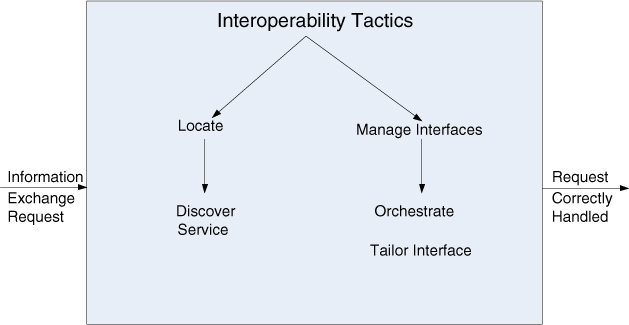
\includegraphics[scale=0.60]{tactic_interoperability.jpg}}
\end{center}


\noindent
With Discover service we will create a clear line between clients and the bulletinboard. We will use a REST to implement a web service for this tactic.\\

\noindent
REST stands for Representation State Transfer. The implementation of REST is as follows. We have a tallycontroller and a votercontroller etc. within the bulletin board, which is build upon the REST design principles. The clients are webclients and they are build on pure javascript. All communcation will be through ajax call to the bulletin board.\\


\noindent
\textbf{Module viewpoint}\\
Show class diagram of the REST "interface".\\

\noindent
\textbf{Component and Connector viewpoint}\\

\noindent
\textbf{Allocation viewpoint}\\


\noindent
\subsubsection{Security}
This tactic is related to QAS 2. Security is concerned with ability to protect data and information from unauthorized access while still providing access to people/systems that are authorized. The PVSS protocol ensures that only valid votes are accepted and counted. This prevents that invalid votes are counted in the final counts and thereby they will not effect the result. The verify message integrity tactic employs techniques such as checksums or hash values to verfy the integrity of a message. After the system has detected an attack the system must react on the attack.

\begin{center}
     \makebox[\textwidth]{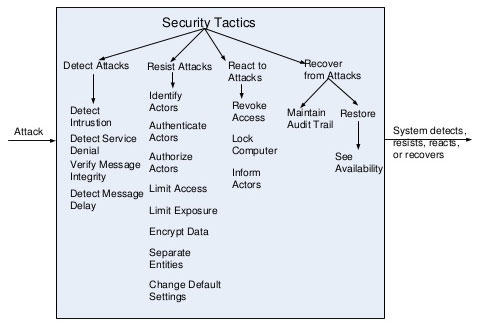
\includegraphics[scale=0.60]{tactic_security.jpg}}
\end{center}
The DLEQ and $PROOF_U$ proofs verifies the message integrity. With the proofs the protocol will be able to detect attacks. The verify message integrity consists of:

\begin{enumerate}
    \item The DLEQ proof provided in ballocasting process ensures consistency in the encryption process.
    \item  The $PROOF_U$ ensures that the voter votes either 0 or 1.
    \item  The DLEQ proof in the tallying process ensures that the decryption is done correct.
\end{enumerate}

\noindent
As already described this tactic is a part of the protocol. Our work consists of realizing the tactic in code. Another important decision to make is if an attack is detected then system, must react. One way could be marking the vote as inactive on the bulletin board and hereafter inform an administrator about the detection of an attack.\\   

\noindent
\textbf{Model viewpoint}\\


\noindent
\textbf{Component and Connector viewpoint}\\
Show sequence diagram of the proofs\\

\noindent
\textbf{Allocation viewpoint}\\


\noindent
\subsubsection{Modifiability}
This tactic is related to QAS 3. Modifiability is concerned with the ease with which the system supports change. To further prove the security of the implementation we must take into account that the random generator easily can be changed. This is an advantage if we need to work with larger numbers in the near further. The encapsulate tactics reduces the coupling between modules. The goal is to create an interface to the number generate so that we are able to shield of the concrete implementation of a given number generator and thereby reduce the coupling between modules. If  we later then need to change the implementation we can create a new implementation of the number generator and  replace the old one. 


\begin{center}
     \makebox[\textwidth]{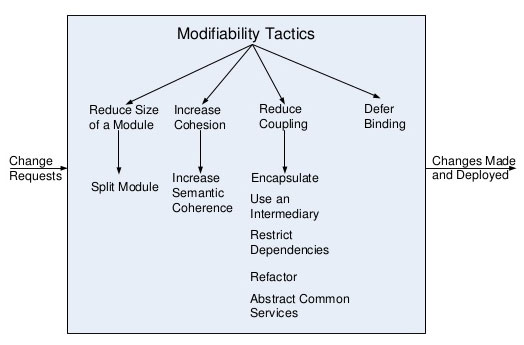
\includegraphics[scale=0.60]{tactic_modifiability.jpg}}
\end{center}

\noindent
This tactic is limited to webclient since they contain all computations and the number generator. The following will be a description of our implementation of the concrete number generator and how we implemented an interface for this number generator in javascript.\\


\noindent
\textbf{Module viewpoint}\\
This viewpoint shows the use of a strategy pattern. The idea with the strategy pattern is to define a family of business rule, encapsulate each one and make them interchangeable. The strategy pattern lets the business rules vary independently from clients that use it. It delegates the responsibility to an object instead of doing the work it self. The VoterClient gets an instance of a randomGen which has a method randBetween. It can either be an instance of a RandomGenStrategy or a FixedNumberStrategy. Each of these classes has their implementation of the method randBetween. The RandomGenStrategy implements the reel random number generator. The FixedNumberStrategy returns a controlled value which we in can be fixed for testing purposes.\\
\begin{center}
     \makebox[\textwidth]{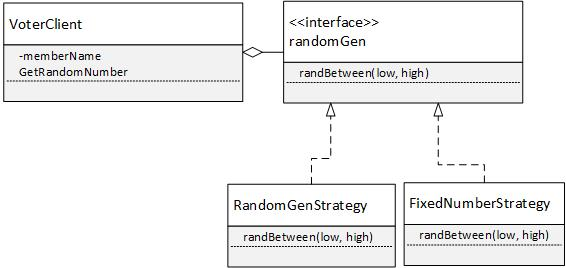
\includegraphics[scale=0.60]{M_View_RandomNumberGenerator.jpg}}
\end{center}






\noindent
\textbf{Component and Connector viewpoint}\\
Insert sequence diagram - delegation p.123\\
\begin{center}
     \makebox[\textwidth]{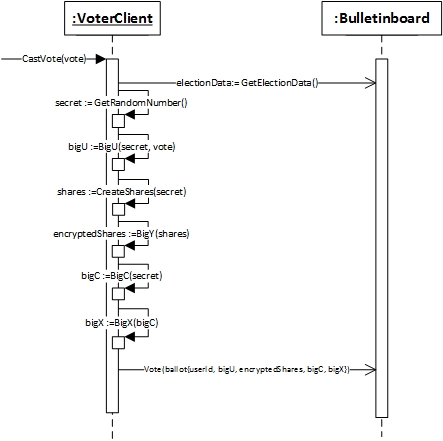
\includegraphics[scale=0.80]{sequenceDiagram_vote.jpg}}
\end{center}

\noindent
\textbf{Allocation viewpoint}\\



\noindent
\subsubsection{Modifiability}
This tactic is related to QAS 4. Modifiability is concerned with the ease with which the system supports change. In a reel electronic voting application scenario there will be need of a certain registration process. Depending on the scenario it could be local municipality. Therefor the system must be able to support changes on the registration process depending on the use.  \\


\noindent
\textbf{Module viewpoint}\\
Class diagram of the registration module. Show strategy pattern\\

\noindent
\textbf{Component and Connector viewpoint}\\

\noindent
\textbf{Allocation viewpoint}\\

\noindent
\subsubsection{Testability}
This tactic is related to QAS 6. Testability is concerned with the ease with which the software can be made to demonstrate its faults. This application contains a fair amount of computation which is the core of the application - namely to compute the final votes. Testing is needed, to ensure accuracy of the computations. When new features are introduced to the system, one should be able to execute all tests and result are captured and 85 \% of the system are coverage within 3 hours.


\begin{center}
     \makebox[\textwidth]{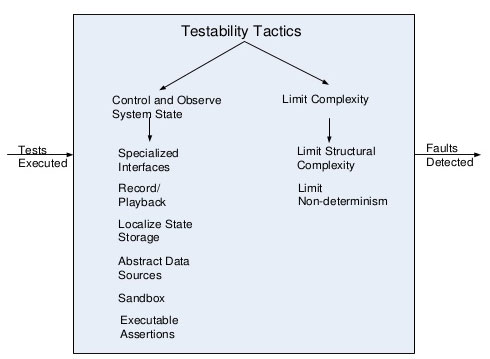
\includegraphics[scale=0.60]{tactic_testability.jpg}}
\end{center}
\noindent
The webclient are build in javascript which means that we have to adapt to the opportunities (dynamic, untyped, and interpreted run-time language) which the language provides. This tactic is limited to webclient since they contain all computations. The tactic limit structural complexity is about isolating, encapsulating dependencies and reduce dependencies between components. These principles leads limited complexity and thereby better testability.   \\

\noindent
\textbf{Module viewpoint}\\
Here we need to talk about jasmine. We need to get static overview of the javascript code.\\

\noindent
\textbf{Component and Connector viewpoint}\\
Sequence diagram\\

\noindent
\textbf{Allocation viewpoint}\\


\subsection{Architectural decision}
This section is about documentation of software architectural decisions and their rationale. The documentation provides a description of choosen architectural decision and the rejected decisions. Another point of describing the idea / rationale behind the decision is that it provides the basis for not making the same stupid mistake again. Tyree and Akerman have made a documentation template that contains the elements for a design decision.


\begin{table}[H]
\centering
\begin{tabular}{|l|l|}
\hline
\multicolumn{2}{|l|}{\textbf{Decision D01:}}                                                                                                                                                                                                                                       \\ \hline
Issue                & \begin{tabular}[c]{@{}l@{}}A PVSS client cast a vote to the Bulletin \\ board from a given device with internet\\  connection, under runtime and the system\\  is updated and 100\% of the information \\ is exchanged,and processed correctly\end{tabular} \\ \hline
Decision             & A REST service is introduced                                                                                                                                                                                                                                \\ \hline
Status               & Pending                                                                                                                                                                                                                                                     \\ \hline
Grouping             &                                                                                                                                                                                                                                                             \\ \hline
Assumptions          &                                                                                                                                                                                                                                                             \\ \hline
Constraints          &                                                                                                                                                                                                                                                             \\ \hline
Positions            &                                                                                                                                                                                                                                                             \\ \hline
Argument             &                                                                                                                                                                                                                                                             \\ \hline
Implications         &                                                                                                                                                                                                                                                             \\ \hline
Related decisions    &                                                                                                                                                                                                                                                             \\ \hline
Related requirements &                                                                                                                                                                                                                                                             \\ \hline
Related artifacts    &                                                                                                                                                                                                                                                             \\ \hline
Related principles   &                                                                                                                                                                                                                                                             \\ \hline
Notes                &                                                                                                                                                                                                                                                             \\ \hline
\end{tabular}
\caption{Interoperability decision}
\label{my-label}
\end{table}


\subsection{Architectural evaluation}